\documentclass{amsart}
%\usepackage[usefamily=sage]{pythontex} 
\usepackage{sagetex}
\usepackage[utf8]{inputenc}
\usepackage{tikz}
\newtheorem{ejer}{Ejercicio}

\def\n{\mathbb{N}}
\def\r{\mathbb{R}}
\def\z{\mathbb{Z}}
\def\q{\mathbb{Q}}
\def\c{\mathbb{C}}


\title{Pr\'acticas de \'Algebra y Matem\'atica Discreta. \\ Bases y Coordenadas}

\begin{document}
\maketitle

\begin{sageblock}
latex.matrix_delimiters("[", "]")
\end{sageblock}

\begin{ejer} Sea $V$ el espacio vectorial cuya base son las columnas de la matriz
\[ B = \left[\begin{array}{rrrrrr}
0 & 2 & 2 & 2 & 3 & 1 \\
4 & 0 & 4 & 6 & 6 & 6 \\
6 & 1 & 5 & 1 & 2 & 3 \\
4 & 3 & 0 & 2 & 6 & 1 \\
2 & 6 & 6 & 4 & 4 & 0 \\
4 & 3 & 5 & 3 & 5 & 5
\end{array}\right] \in {\bf M}_{6 \times 6}({\mathbb Z}_{7})\]
Determina si el vector $y = {\left[\begin{array}{r}
2 \\
2 \\
1 \\
5 \\
0 \\
4
\end{array}\right]}$ est\'a en $V$ y en caso de estarlo, calcula sus coordenadas 
en base $B$.
\end{ejer}

{\it Soluci\'on:}
% Escribe tu soluci\'on para el Ejercicio 1

\begin{sageblock}
B=matrix(Zmod(7),[[0,2,2,2,3,1],[4,0,4,6,6,6],
[6,1,5,1,2,3],[4,3,0,2,6,1],
[2,6,6,4,4,0],[4,3,5,3,5,5]])
y=column_matrix(Zmod(7),[2,2,1,5,0,4])
By = block_matrix(1,2,[B,y])
R=By.echelon_form()
\end{sageblock}

El vector $y$ está en $V=C(B)$ si es combinación lineal de las columnas de la 
matriz $B$. Ello equivale a que el sistema de ecuaciones $B\cdot x = y$ es compatible.

Determinamos la matriz ampliada

$$ \sage{By} $$

Reducimos por filas

$$ \sage{R} $$

Como la columna de términos independientes no es pivote, el sistema es compatible 
y el vector $y$ está en $V$. Además se tiene que

$$ y = \sage{y} = {\sage{R.subdivision(0,1)}}_B $$

% Fin del Ejercicio 1

\begin{ejer} Sea $V$ el espacio vectorial cuya base son las columnas de la matriz
\[ B = \left[\begin{array}{rrr}
1 & -2 & -5 \\
0 & 1 & 3 \\
3 & -4 & -8 \\
-1 & 0 & 4\\
1 & -4 & -6
\end{array}\right] \in {\bf M}_{5 \times 3}(\r )\]
Determina si el vector $y = {\left[\begin{array}{r}
-5 \\
3 \\
-8 \\
4 \\
-5
\end{array}\right]}$ est\'a en $V$ y en caso de estarlo, calcula sus coordenadas 
en base $B$.
\end{ejer}
{\it Soluci\'on:}
% Escribe tu soluci\'on para el Ejercicio 2


% Fin del Ejercicio 2

\begin{ejer} Sea $V$ un espacio vectorial del cual conocemos dos bases, $B$ y 
$B'$ que corresponden a las columnas de las siguientes matrices
\[ B' = \left[\begin{array}{rrr}
15 & -8 & -38 \\
2 & -1 & -6 \\
-10 & 5 & 31 \\
4 & -2 & -14 \\
8 & -4 & -23 \\
0 & 0 & -3
\end{array}\right] , B = \left[\begin{array}{rrr}
1 & 7 & -1 \\
0 & 1 & -1 \\
0 & -5 & 6 \\
0 & 2 & -4 \\
0 & 4 & -3 \\
0 & 0 & -3
\end{array}\right] \in {\bf  M}_{6 \times 3}({\mathbb R})\]
Calcula la matriz de cambio de base $P_{B'B}$.
\end{ejer}

{\it Soluci\'on:}
% Escribe tu soluci\'on para el Ejercicio 3

Dadas las bases $B$ y $B'$ sabemos que la matriz del cambio $P_{B'B}$ es la 
matriz $A\cdot B'$ donde $A$ es una inversa lateral por la izquierda de $B$.

\begin{sageblock}
B=matrix(QQ,[[1,7,-1],[0,1,-1],
[0,-5,6],[0,2,-4],
[0,4,-3],[0,0,-3]])
B1=matrix(QQ,[[15,-8,-38],[2,-1,-6],
[-10,5,31],[4,-2,-14],
[8,-4,-23],[0,0,-3]])
BI = block_matrix(1,2,[B,1])
R=BI.echelon_form()
R=copy(R)
R.subdivide(3,3)
A=R.subdivision(0,1)
\end{sageblock}

Pasamos a determinar una inversa lateral por la izquierda de la matriz $B$. Para 
ello ampliamos a la derecha de la matriz $B$ con la identidad

$$ \sage{BI} $$

Reducimos por filas dicha matriz 

$$ \sage{R} $$

Una inversa lateral por la izquierda de $B$ es la matriz $A$, donde

$$ A = \sage{A} $$

Por tanto

$$ P_{B'B} = \sage{A}\cdot \sage{B1} = \sage{A*B1} $$

Este problema es equivalente a calcular la matriz de la aplicación lineal 
$$
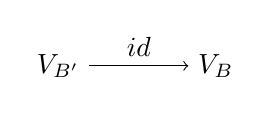
\begin{tikzpicture}
\node (VBp) at (0,0) {$V_{B'}$};
\node (VB) at (2,0) {$V_B$};
\draw[->] (VBp) to node [above] {$id$} (VB);
\end{tikzpicture}
$$
y podemos aplicar la fórmula 
$$P_{B'B} = M_{B'B}(id) = A ~ id(B') = AB' = \sage{A*B1}.$$

% Fin del Ejercicio 3

\begin{ejer} Sea $V$ un espacio vectorial del cual conocemos la base $B$  
que corres\-ponden a las columnas de la matriz
\[ B = \left[\begin{array}{rrrr}
1 & 7 & -1 & 2 \\
0 & 1 & -1 & -1 \\
0 & -5 & 6 & -4 \\
0 & 2 & -4 & -1
\end{array}\right] \in {\bf  M}_{4 \times 4}({\z _7})\]
Calcula la matriz de cambio de base $P_{C_4B}$.
\end{ejer}

{\it Soluci\'on:}
% Escribe tu soluci\'on para el Ejercicio 4

\begin{sageblock}
B=matrix(Zmod(7),[[1,7,-1,2],[0,1,-1,-1],
[0,-5,6,-4],[0,2,-4,-1]])
\end{sageblock}

Tenemos el siguiente diagrama:
$$
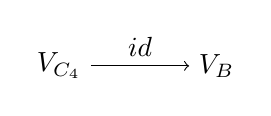
\begin{tikzpicture}
\node (VC) at (0,0) {$V_{C_4}$};
\node (VB) at (2,0) {$V_B$};
\draw[->] (VC) to node [above] {$id$} (VB);
\end{tikzpicture}
$$

En general, la matriz del cambio de base es la inversa por la izquierda de
$B$ por la matriz de $C_4$. Como $B$ es cuadrada, su inversa por la izquierda
es su inversa normal y la matriz asociada a la base canónica es la identidad,
por tanto $$P_{C_4B} = B^{-1} I = \sage{B^-1}.$$

% Fin del Ejercicio 4


\begin{ejer} Sea la aplicación $f: \r ^3\to \r ^3$ tal que 
\[ M(f) = \left[ \begin{array}{rrr} 1 & 2 & 3\\ -3 & -5 & -8\\ 
-1 & -5 & -6 \end{array} \right]. \] Si $B'$ y $B$ son bases 
dadas por las matrices 
\[ B' = \left[ \begin{array}{rrr} 1 & 1 & 6\\ -1 & 0 & -2\\ 
0 & 0 & 1 \end{array} \right] \ \hbox{y} \ B = 
\left[ \begin{array}{rrr} -2 & 7 & 3\\ 1 & -4 & -1\\ 
0 & 0 & 1 \end{array} \right],  \] Calcula $M_{B'B}(f)$.
\end{ejer}

{\it Soluci\'on:}
% Escribe tu soluci\'on para el Ejercicio 5

\begin{sageblock}
Mf = matrix(QQ,[[1,2,3],[-3,-5,-8],[-1,-5,-6]])
B1=matrix(QQ,[[1,1,6],[-1,0,-2],[0,0,1]])
B=matrix(QQ,[[-2,7,3],[1,-4,-1],[0,0,1]])
\end{sageblock}

Consideremos el siguiente diagrama:

$$
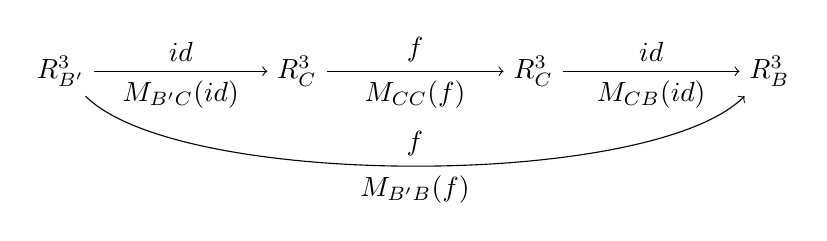
\begin{tikzpicture}[xscale = 1.5]
\node (RBp) at (0,0) {$\r^3_{B'}$};
\node (RCa) at (2,0) {$\r^3_C$};
\node (RCb) at (4,0) {$\r^3_C$};
\node (RB)  at (6,0) {$\r^3_B$};
\draw[->] (RBp) to node [above] {$id$} 
                   node [below] {$M_{B'C}(id)$} (RCa);
\draw[->] (RCa) to node [above] {$f$} node [below] {$M_{CC}(f)$} (RCb); 
\draw[->] (RCb) to node [above] {$id$} node [below] {$M_{CB}(id)$} (RB);
\draw[->] (RBp) .. controls (1,-1.5) and (5,-1.5) .. 
                   node [above] {$f$} 
                   node [below] {$M_{B'B}(f)$} (RB);
\end{tikzpicture}
$$

Si calculamos cada una de las matrices de esas aplicaciones tenemos que
\begin{itemize}
\item $M_{CB}(id) = P_{CB} = B^{-1}I = B^{-1}$ porque $B$ es cuadrada
y su inversa por la izquierda es su inversa.
\item $M_{CC}(f) = M(f)$ nos la dan.
\item $M_{B'C}(id) = P_{B'C} = I^{-1}B'= B'$ porque la matriz asociada a la
base canónica es la matriz identidad, que es cuadrada y su inversa 
es ella misma. 
\end{itemize}

Por lo tanto
\[ M_{B'B}(f) = B^{-1}M(f)B' = \] \[ \sage{B^-1}\sage{Mf}\sage{B1} = 
\sage{B^-1*Mf*B1}. \]

% Fin del Ejercicio 5

\begin{ejer} 
Sea la aplicación $f: \r ^4\to \r ^3$ tal que 
\[ M_{B'B}(f) = \left[ \begin{array}{rrrr} -2 & -6 & 2 & 0 \\ -3 & -9 & 3 & 0 \end{array} \right] \] siendo $B'$ y $B$ las bases dadas por las matrices 
\[ B' = \left[ \begin{array}{rrrr} 6 & -4 & 0 & 3\\ -1 & 2 & -4 & -7\\ 
0 & 2 & -5 & -7\\ 5 & -3 & -1 & 1 \end{array} \right] \ \hbox{y} \ B = \left[ \begin{array}{rr} -1 & 5\\ -2 & 9 \end{array} \right],  \] 
Calcula $M(f)$.
\end{ejer}

{\it Soluci\'on:}
% Escribe tu soluci\'on para el Ejercicio 6
\begin{sageblock}
MB1Bf = matrix(QQ,[[-2,-6,2,0],[-3,-9,3,0]])
B1=matrix(QQ,[[6,-4,0,3],[-1,2,-4,-7],[0,2,-5,-7],[5,-3,-1,1]])
B=matrix(QQ,[[-1,5],[-2,9]])
\end{sageblock}

Consideremos el siguiente diagrama:

$$
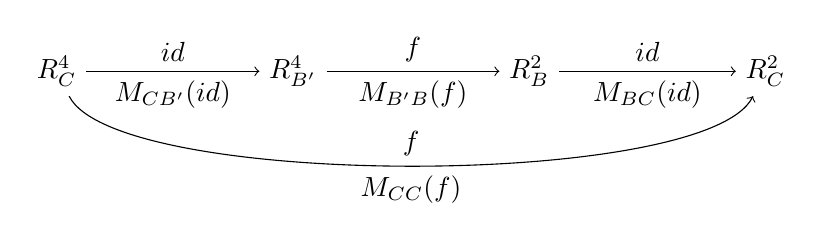
\begin{tikzpicture}[xscale = 1.5]
\node (RCa) at (0,0) {$\r^4_C$};
\node (RBp) at (2,0) {$\r^4_{B'}$};
\node (RB)  at (4,0) {$\r^2_B$};
\node (RCb) at (6,0) {$\r^2_C$};
\draw[->] (RCa) to node [above] {$id$} 
                   node [below] {$M_{CB'}(id)$} (RBp);
\draw[->] (RBp) to node [above] {$f$} 
                   node [below] {$M_{B'B}(f)$} (RB); 
\draw[->] (RB)  to node [above] {$id$} 
                   node [below] {$M_{BC}(id)$} (RCb);
\draw[->] (RCa) .. controls (0.5,-1.5) and (5.5,-1.5) .. 
                node [below] {$M_{CC}(f)$} 
                node [above] {$f$} (RCb);
\end{tikzpicture}
$$

Si calculamos cada una de las matrices de esas aplicaciones tenemos que
\begin{itemize}
\item $M_{CB'}(id) = P_{CB'} = (B')^{-1}I = (B')^{-1}$.
\item $M_{B'B}(f)$ nos la dan.
\item $M_{BC}(id) = P_{BC} = I^{-1}B= B$. 
\end{itemize}

De donde 
\[ M(f) = M_{CC}(f) = M_{BC}(id) \ M_{B'B}(f) \ M_{CB'}(id) = B \ M_{B'B}(f) \ (B')^{-1} = \] 
\[ \sage{B}\sage{MB1Bf}\sage{B1.inverse()} \] 
\[ = \sage{B*MB1Bf*B1.inverse()}. \]

% Fin del Ejercicio 6


\begin{ejer} 
Sea la aplicación $f: \r^2\to \r^4$ tal que 
\[ M_{C_2B_1}(f) = \left[ \begin{array}{rr} -2 & -8 \\ 2 & 9 \\ -1 & -4 \\ 
-1 & -1 \end{array} \right]. \] Calcula $M_{C_2B_2}(f)$ siendo $B_1$ y $B_2$ 
las bases dadas por las matrices 
\[ B_1 = \left[ \begin{array}{rrrr} 1 & 1 & -2 & -2\\ 1 & 2 & -3 & -4\\ 
1 & -1 & 1 & 5\\ -4 & -1 & 7 & 9 \end{array} \right] \ \hbox{y} \ 
B_2 = \left[ \begin{array}{rrrr} 1 & 2 & -1 & 8\\ 0 & 1 & -1 & 0\\ 
0 & 5 & -4 & 5\\ 0 & 5 & -6 & -4 \end{array} \right].  \]
\end{ejer}

{\it Soluci\'on:}
% Escribe tu soluci\'on para el Ejercicio 7

Para pintar el diagrama puedes usar como base el siguiente dibujo:

$$
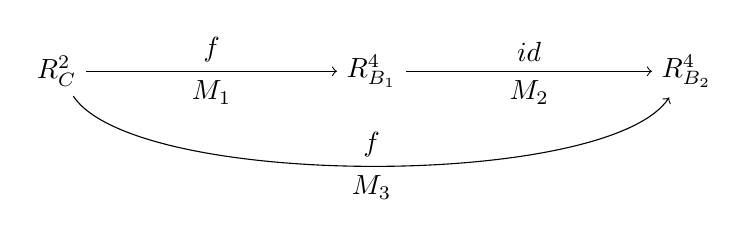
\begin{tikzpicture}[xscale = 2]
\node (RC)  at (0,0) {$\r^2_C$};
\node (RB1) at (2,0) {$\r^4_{B_1}$};
\node (RB2) at (4,0) {$\r^4_{B_2}$};
\draw[->] (RC)  to node [above] {$f$} 
                   node [below] {$M_1$} (RB1);
\draw[->] (RB1) to node [above] {$id$} 
                   node [below] {$M_2$} (RB2); 
\draw[->] (RC) .. controls (0.5,-1.5) and (3.5,-1.5) .. 
               node [above] {$f$}
               node [below] {$M_3$} (RB2);
\end{tikzpicture}
$$


% Fin del Ejercicio 7

\begin{ejer} 
Sea la aplicación $f: \r ^3\to \r ^2$ tal que 
\[ M_{B_1C}(f) = \left[ \begin{array}{rrr} 4 & 0 & 8 \\  
3 & 0 & 6 \end{array} \right]. \] Calcula $M_{B_2C}(f)$ 
siendo $B_1$ y $B_2$ las bases dadas por las matrices 
\[ B_1 = \left[ \begin{array}{rrr} -2 & 3 & -5\\ 3 & -5 & 8\\ 0 & -4 & 5 
\end{array} \right] \ \hbox{y} \ B_2 = \left[ \begin{array}{rrr} 1 & 1 & -2\\ 
3 & 4 & -8\\ -5 & -3 & 7  \end{array} \right].  \]
\end{ejer}

{\it Soluci\'on:}
% Escribe tu soluci\'on para el Ejercicio 8

\begin{sageblock}
MB11C2f = matrix(QQ,[[4,0,8],[3,0,6]])
B11=matrix(QQ,[[-2,3,-5],[3,-5,8],[0,-4,5]])
B12=matrix(QQ,[[1,1,-2],[3,4,-8],[-5,-3,7]])
\end{sageblock}

Consideremos el siguiente diagrama:

$$
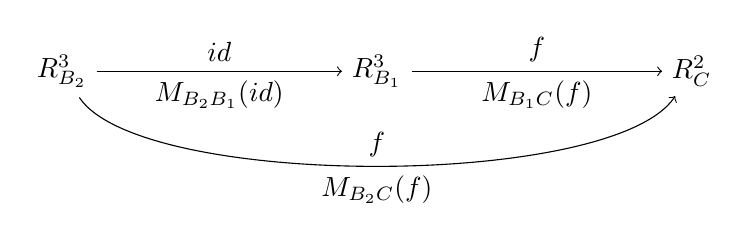
\begin{tikzpicture}[xscale = 2]
\node (RB2) at (0,0) {$\r^3_{B_2}$};
\node (RB1) at (2,0) {$\r^3_{B_1}$};
\node (RC)  at (4,0) {$\r^2_{C}$};
\draw[->] (RB2) to node [above] {$id$} 
                   node [below] {$M_{B_2B_1}(id)$} (RB1);
\draw[->] (RB1) to node [above] {$f$} 
                   node [below] {$M_{B_1C}(f)$} (RC); 
\draw[->] (RB2) .. controls (0.5,-1.5) and (3.5,-1.5) .. 
                node [above] {$f$}
                node [below] {$M_{B_2C}(f)$} (RC);
\end{tikzpicture}
$$

Si calculamos cada una de las matrices de esas aplicaciones tenemos que
\begin{itemize}
\item $M_{B_2B_1}(id) = B_1^{-1} B_2$ porque $B_1$ es cuadrada
y su inversa por la izquierda es su inversa.
\item $M_{B_1C}(f)$ nos la dan. 
\end{itemize}

Entonces 
\[ M_{B_2C}(f) = M_{B_1C}(f) \ M_{B_2B_1}(id) = \] 
\[   \sage{MB11C2f}{\sage{B11}}^{-1}\sage{B12} \] 
\[ = \sage{MB11C2f*B11.inverse()*B12}. \]

% Fin del Ejercicio 8

\begin{ejer} 
Sea la aplicación $f: \r ^2\to \r ^2$ tal que 
\[ M_{B'B}(f) = \left[ \begin{array}{rr} -2 & 2 \\  -1 & 1 \end{array} \right], \]  siendo $B'$ y $B$ las bases dadas por las matrices 
\[ B' = \left[ \begin{array}{rr} 6 & -5\\ 5 & -4 \end{array} \right] \ \hbox{y} \ B = \left[ \begin{array}{rr} -1 & -5\\ 2 & 9  \end{array} \right].  \] Calcula $M(f)$.
\end{ejer}

{\it Soluci\'on:}
% Escribe tu soluci\'on para el Ejercicio 9

\begin{sageblock}
MB1Bf = matrix(QQ,[[-2,2],[-1,1]])
B1=matrix(QQ,[[6,-5],[5,-4]])
B=matrix(QQ,[[-1,-5],[2,9]])
\end{sageblock}

Consideremos el siguiente diagrama:

$$
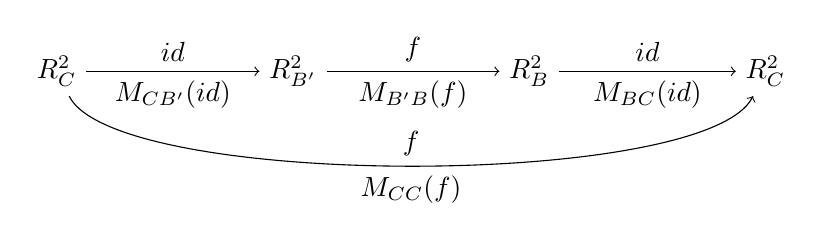
\begin{tikzpicture}[xscale = 1.5]
\node (RCa) at (0,0) {$\r^2_C$};
\node (RBp) at (2,0) {$\r^2_{B'}$};
\node (RB)  at (4,0) {$\r^2_B$};
\node (RCb) at (6,0) {$\r^2_C$};
\draw[->] (RCa) to node [above] {$id$} 
                   node [below] {$M_{CB'}(id)$} (RBp);
\draw[->] (RBp) to node [above] {$f$} 
                   node [below] {$M_{B'B}(f)$} (RB); 
\draw[->] (RB)  to node [above] {$id$} 
                   node [below] {$M_{BC}(id)$} (RCb);
\draw[->] (RCa) .. controls (0.5,-1.5) and (5.5,-1.5) .. 
                node [below] {$M_{CC}(f)$} 
                node [above] {$f$} (RCb);
\end{tikzpicture}
$$

Si calculamos cada una de las matrices de esas aplicaciones tenemos que
\begin{itemize}
\item $M_{CB'}(id) = P_{CB'} = (B')^{-1}I = (B')^{-1}$ porque $B'$ es cuadrada
y su inversa por la izquierda es su inversa.
\item $M_{B'B}(f)$ nos la dan.
\item $M_{BC}(id) = P_{BC} = I^{-1}B= B$. 
\end{itemize}

De donde 
\[ M(f) = M_{CC}(f) = M_{CC}(id\circ f\circ id) =  M_{BC}(id) \ 
M_{B'B}(f) \ M_{CB'}(id) = \] 
\[ \sage{B}\sage{MB1Bf}{\sage{B1}}^{-1} = \sage{B*MB1Bf*B1.inverse()}. \]

% Fin del Ejercicio 9


\begin{ejer} 
Sea la aplicación $f: \z _5^2\to \z _5^3$ tal que 
\[ M_{B'C}(f) = \left[ \begin{array}{rr} 2 & 3 \\ 4 & 4\\ 
1 & 3 \end{array} \right], \]  Calcula $M_{C_2B}(f)$. siendo $B'$ y $B$ las bases 
dadas por las matrices 
\[ B' = \left[ \begin{array}{rr} 6 & -5\\ 5 & -4 \end{array} \right] 
\ \hbox{y} \ B = \left[ \begin{array}{rrr} 2 & 3 & 4\\ 0 & -3 & 4\\ 
0 & 0 & 3 \end{array} \right].  \]
\end{ejer}

{\it Soluci\'on:}
% Escribe tu soluci\'on para el Ejercicio 10
\begin{sageblock}
MB1C3f = matrix(Zmod(5),[[2,3],[4,4],[1,3]])
B1=matrix(Zmod(5),[[6,-5],[5,-4]])
B=matrix(Zmod(5),[[2,3,4],[0,-3,4],[0,0,3]])
\end{sageblock}

Consideremos el siguiente diagrama:

$$
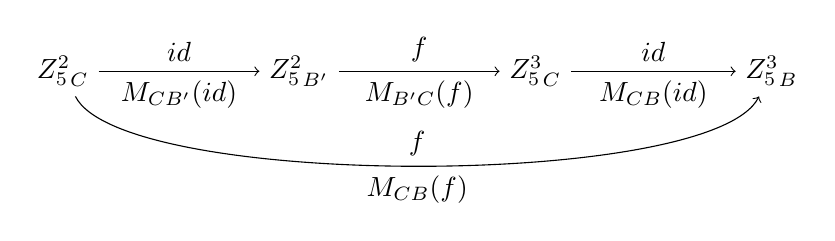
\begin{tikzpicture}[xscale = 1.5]
\node (ZCa) at (0,0) {${\z _5^2}_C$};
\node (ZBp) at (2,0) {${\z _5^2}_{B'}$};
\node (ZCb) at (4,0) {${\z _5^3}_C$};
\node (ZB)  at (6,0) {${\z _5^3}_B$};
\draw[->] (ZCa) to node [above] {$id$} 
                   node [below] {$M_{CB'}(id)$} (ZBp);
\draw[->] (ZBp) to node [above] {$f$} 
                   node [below] {$M_{B'C}(f)$} (ZCb); 
\draw[->] (ZCb)  to node [above] {$id$} 
                   node [below] {$M_{CB}(id)$} (ZB);
\draw[->] (ZCa) .. controls (0.5,-1.5) and (5.5,-1.5) .. 
                node [below] {$M_{CB}(f)$} 
                node [above] {$f$} (ZB);
\end{tikzpicture}
$$

Si calculamos cada una de las matrices de esas aplicaciones tenemos que
\begin{itemize}
\item $M_{CB'}(id) = P_{CB'} = (B')^{-1}I = (B')^{-1}$.
\item $M_{B'C}(f)$ nos la dan.
\item $M_{CB}(id) = P_{CB} = B^{-1}I= B^{-1}$. 
\end{itemize}

De donde 
\[ M_{CB}(f) = M_{CB}(id\circ f\circ id) =  M_{CB}(id) M_{B'C}(f) M_{CB'}(id) \] 
\[ = {\sage{B}}^{-1}\sage{MB1C3f}{\sage{B1}}^{-1} = \sage{B.inverse()*MB1C3f*B1.inverse()}. \]

% Fin del Ejercicio 10


\begin{ejer} Calcula una base del espacio $N(A)$, anulador por la derecha de $A$ siendo $A$ la matriz
\[ \left[\begin{array}{rrrr}
1 & 1 & 1 & 2 \\
1 & 0 & 2 & 0 \\
0 & 1 & 2 & 2 
\end{array}\right] \in {\bf M}_{3 \times 4}({\mathbb Z}_{3})\]
\end{ejer}

{\it Soluci\'on:}
% Escribe tu soluci\'on para el Ejercicio 11
\begin{sageblock}
A=matrix(Zmod(3),[[1,1,1,2],[1,0,2,0],[0,1,2,2]])
R = A.echelon_form()
P = PolynomialRing(Zmod(3),4,'x')
X = matrix(P,4,1,P.gens())
Ecuaciones = A*X
EcuacionesR = R*X
v1 = column_matrix(Zmod(3),[1,1,1,0])
v2 = column_matrix(Zmod(3),[0,1,0,1])
\end{sageblock}

$N(A)$ es el conjunto de soluciones del sistema
$$ \sage{A} \sage{X} = 0 $$
que escrito en forma de ecuaciones es

\begin{align*}
\sage{Ecuaciones[0,0]} &= 0 \\
\sage{Ecuaciones[1,0]} &= 0 \\
\sage{Ecuaciones[2,0]} &= 0 \\
\end{align*}

Si reducimos por filas otenemos 
$$ \sage{R}$$
que corresponde al sistema de ecuaciones
\begin{align*}
\sage{EcuacionesR[0,0]} &= 0 \\
\sage{EcuacionesR[1,0]} &= 0 \\
\sage{EcuacionesR[2,0]} &= 0 \\
\end{align*}
Si tomamos como parámetros las variables $x_2 = a$ y $x_3 = b$ podemos
escribir las soluciones como 
$$ \sage{X} = a \sage{v1} + b \sage{v2} $$
Esto nos da la base que buscamos 
$$ \left\{ \sage{v1}, \sage{v2} \right\} $$

% Fin del Ejercicio 11

\begin{ejer} Calcula una base de $C(A)$, espacio generado por las columnas de $A$ siendo $A$ la matriz
\[ \left[\begin{array}{rrr}
4 & 4 & 2 \\
2 & 1 & 0 \\
2 & 2 & 2 
\end{array}\right] \in {\bf M}_{3 \times 3}({\mathbb Z}_{5})\]
\end{ejer}

{\it Soluci\'on:}
% Escribe tu soluci\'on para el Ejercicio 12
\begin{sageblock}
A = matrix(Zmod(5),[[4,4,2],[2,1,0],[2,2,2]])
R = A.echelon_form()
\end{sageblock}
Debemos encontrar el máximo número de columnas linealmente independientes. 
Reducimos la matriz $A$ (bastaría con triangularizar) y obtenemos
\[ \sage{R} \] Todas las columnas son columnas pivote. Las columnas de la 
matriz original forman la base buscada:

\[ \left\lbrace \sage{A[:,0]}, \sage{A[:,1]}, \sage{A[:,2]}  \right\rbrace \]


% Fin del Ejercicio 12


\begin{ejer} Calcula una base de $C(A^T)$, espacio generado por las filas de $A$, siendo $A$ la matriz
\[ \left[\begin{array}{rrrr}
0 & 4 & 3 & 1 \\
1 & 0 & 2 & 0 \\
3 & 3 & 3 & 0 
\end{array}\right] \in {\bf M}_{3 \times 4}({\mathbb Z}_{5})\]
\end{ejer}

{\it Soluci\'on:}
% Escribe tu soluci\'on para el Ejercicio 13
\begin{sageblock}
A=matrix(Zmod(5),[[0,4,3,1],[1,0,2,0],[3,3,3,0]])
B=A.echelon_form()
\end{sageblock}
Para ello vamos a combinar las filas de $A$ para conseguir vectores 
linealmente independientes. Obtenemos
\[ \sage{B} \] La base es:
\[ \left\lbrace \sage{B[0,:].T}, \sage{B[1,:].T}, \sage{B[2,:].T} \right\rbrace \] 

%Fin del Ejercicio 13

\begin{ejer} Calcula una base de $N(A^T)$, espacio anulador por la izquierda de 
$A$, siendo $A$ la matriz
\[ \left[\begin{array}{rr}
0 & 2 \\
0 & 1 \\
2 & 0 \\ 
2 & 1 
\end{array}\right] \in {\bf M}_{4 \times 2}({\mathbb Z}_{5})\]
\end{ejer}

{\it Soluci\'on:}
% Escribe tu soluci\'on para el Ejercicio 14
\begin{sageblock}
A=matrix(Zmod(3),[[0,2],[0,1],[2,0],[2,1]])
B=block_matrix(1,2,[A,1])
R=B.echelon_form()
R=copy(R)
R.subdivide(2,2)
H = R.subdivision(1,1)
\end{sageblock}
Para ello vamos y puesto que sólo nos interesa detectar las filas de ceros 
reducimos la matriz extendida con la matriz identidad: 
$$\sage{B} \to \sage{R}. $$
Si nos quedamos con las filas a la derecha de las filas nulas de la reducción, 
la base es:
\[ \left\lbrace \sage{H[0,:].T}, \sage{H[1,:].T}  \right\rbrace   \] 


%Fin del Ejercicio 14

\begin{ejer} Sea $V = C(B)$ el espacio generado por las columnas de la matriz
\[ B = \left[\begin{array}{rrrr}
3 & 4 & 4 & 0 \\
1 & 0 & 0 & 0 \\
4 & 2 & 3 & 3 
\end{array}\right] \in {\bf M}_{3 \times 4}({\mathbb Z}_{5})\] Extrae una base de entre los vectores columna de $B$.
\end{ejer}
{\it Soluci\'on:}
% Escribe tu soluci\'on para el Ejercicio 15
\begin{sageblock}
B=matrix(Zmod(5),[[3,4,4,0],[1,0,0,0],[4,2,3,3]])
C=B.echelon_form()
\end{sageblock}
Para encontrar la base debemos encontrar el máximo número de columnas libres es 
decir pivote. Reducimos $B$ (bastaría con triangularizar) y obtenemos
\[ \sage{C} \] Las columnas pivote son $1$, $2$ y $3$, por lo tanto la base es
\[ \left\lbrace \sage{B[:,0]}, \sage{B[:,1]}, \sage{B[:,2]}  \right\rbrace \] 

%Fin del Ejercicio 15

\begin{ejer} Sea $V$ un espacio vectorial con base $B$ y consideremos los 
vectores linealmente independientes de $V$ dados por las columnas de $B'$.
Extiende $B'$ usando columnas de $B$ para formar una base de $V$, siendo 
\[B = \left[\begin{array}{rr}
1 & -4 \\
-1 & 5 \\
-3 & 7 \\
1 & -2
\end{array}\right] \in {\bf M}_{4 \times 2}({\mathbb R}) \qquad
B' = \left[\begin{array}{r}
5 \\
-6 \\
-10 \\
3
\end{array}\right] \in {\bf M}_{4 \times 1}({\mathbb R}) \]
\end{ejer}

{\it Soluci\'on:}
% Escribe tu soluci\'on para el Ejercicio 16
\begin{sageblock}
B=matrix(QQ,[[1,-4],[-1,5],[-3,7],[1,-2]])
B1=column_matrix(QQ,[5,-6,-10,3])
B1B=block_matrix(1,2,[B1,B])
C=B1B.echelon_form()
\end{sageblock}

La base que nos piden la obtendremos a través del conjunto generador de $V$ dado 
por los vectores $[B'|B]$. Al reducirla (bastaría con triangularizar) obtenemos
\[ \sage{C}. \]  Las columnas pivote son $1$ y $2$, por lo que esas son precisamente 
las columnas de $[B'|B]$ que son base buscada:
\[ \left\lbrace \sage{B1B[:,0]}, \sage{B1B[:,1]}  \right\rbrace \] 

% Fin del Ejercicio 16

\begin{ejer} Sea $V = C(B)$ y $U = C(B')$. Determina si el espacio $U$ es un subespacio de $V$, siendo 
\[B = \left[\begin{array}{rrrrr}
0 & 3 & 2 & 4 \\
3 & 1 & 0 & 1 \\
3 & 0 & 2 & 4 \\
0 & 0 & 3 & 3 \\
2 & 4 & 2 & 1
\end{array}\right] \in {\bf M}_{5 \times 4}({\mathbb Z}_{5}) \qquad
B' = \left[\begin{array}{rrrrr}
2 & 4 \\
2 & 4 \\
0 & 2 \\
1 & 3 \\
2 & 3
\end{array}\right] \in {\bf M}_{5 \times 2}({\mathbb Z}_{5}) \]
\end{ejer}

{\it Soluci\'on:}
% Escribe tu soluci\'on para el Ejercicio 17
Si $V=C(B)$ y $U=C(B')$, entonces $U\subseteq V$ si y sólo si todas las columnas 
de $B'$ se pueden expresar como combinación lineal de las columnas de $B$, lo 
que equivale a que al reducir por filas la matriz $[B|B']$, las columnas de $B'$ 
no son columnas pivote.

\begin{sageblock}
B=matrix(Zmod(5),[[0,3,2,4],[3,1,0,1],
[3,0,2,4],[0,0,3,3],[2,4,2,1]])
B1=matrix(Zmod(5),[[2,4],[2,4],
[0,2],[1,3],[2,3]])
BB1 = block_matrix(1,2,[B,B1])
R=BB1.echelon_form()
\end{sageblock}

Ampliamos la matriz $B$ a su derecha con la matriz $B'$.

$$ [B|B'] = \sage{BB1} $$

Reduciendo por filas obtenemos la matriz (sobraría con triangularizar)

$$ \sage{R} $$

Vemos que ninguna columna de la matriz $B'$ es pivote, por lo tanto todos los 
vectores de $B'$ están en $V$ y $U \leq V$.

% Fin del Ejercicio 17


\begin{ejer} Sea $V = C(B)$ y $U = C(B')$. Determina si el espacio $U$ es un 
subespacio de $V$, siendo 
\[B = \left[\begin{array}{rrrrr}
3 & 0 & 4 & 1 & 3 \\
6 & 6 & 4 & 4 & 2 \\
4 & 0 & 5 & 0 & 0 \\
6 & 3 & 1 & 0 & 1 \\
4 & 5 & 4 & 0 & 0 \\
1 & 6 & 3 & 0 & 3
\end{array}\right] \in {\bf M}_{6 \times 5}({\mathbb Z}_{7}) \qquad
B' = \left[\begin{array}{rrrrr}
2 & 3 & 2 & 3 & 6 \\
6 & 6 & 1 & 3 & 1 \\
0 & 2 & 6 & 0 & 5 \\
4 & 5 & 4 & 3 & 5 \\
2 & 2 & 1 & 5 & 6 \\
3 & 0 & 3 & 0 & 5
\end{array}\right] \in {\bf M}_{6 \times 5}({\mathbb Z}_{7}) \]
\end{ejer}

{\it Soluci\'on:}
% Escribe tu soluci\'on para el Ejercicio 18



% Fin del Ejercicio 18

\begin{ejer} Sea $V = N(H)$ y $U = N(H')$. Determina si el espacio $V$ es un subespacio de $U$, siendo 
\[H = \left[\begin{array}{rrrrr}
1 & 4 & 4 & 2 & 0 \\
0 & 2 & 4 & 2 & 4 \\
2 & 1 & 4 & 2 & 1 \\
2 & 2 & 1 & 3 & 3
\end{array}\right] \in {\bf M}_{4 \times 5}({\mathbb Z}_{5}) \qquad
H' = \left[\begin{array}{rrrrr}
4 & 2 & 3 & 4 & 2 \\
1 & 1 & 3 & 4 & 4 
\end{array}\right] \in {\bf M}_{2 \times 5}({\mathbb Z}_{5}) \]
\end{ejer}

{\it Soluci\'on:}
% Escribe tu soluci\'on para el Ejercicio 19
\begin{sageblock}
H=matrix(Zmod(5),[[1,4,4,2,0],[0,2,4,2,4],
[2,1,4,2,1],[2,2,1,3,3]])
H1=matrix(Zmod(5),[[4,2,3,4,2],[1,1,3,4,4]])
HTI = block_matrix(1,2,[H.T,1])
R=HTI.echelon_form()
R=copy(R)
R.subdivide(2,4)
A=R.subdivision(1,1)
\end{sageblock}

Para ver si $V$ es un subespacio de $U$, pasamos $V$ a paramétricas, $V=C(A)$. 
Entonces como $V=C(A)$ y $U=N(H')$, $V\leq U$ si y sólo si $H'\cdot A = 0$.

Determinamos la matriz $[H^T|I]$

$$ [H^T|I] =  \sage{HTI} $$

Reducimos por filas

$$ \sage{R} $$

Las paramétricas de $V$ son $V = C(A)$ donde $A$ es la matriz

$$ A = \sage{A.T} $$


$$ H'\cdot A = \sage{H1}\cdot \sage{A} = \sage{H1*A.T} $$ Como el resultado es $0$, concluimos que $V\leq U$.

% Fin del Ejercicio 19


\begin{ejer} Sea $V = N(H)$ y $U = N(H')$. Determina si el espacio $V$ es un subespacio de $U$, siendo 
\[H = \left[\begin{array}{rrrrr}
12 & 19 & 9 & 30 & 0 \\
30 & 14 & 29 & 4 & 19 \\
28 & 14 & 11 & 29 & 28 \\
3 & 1 & 12 & 25 & 13
\end{array}\right] \in {\bf M}_{4 \times 5}({\mathbb Z}_{31}) \qquad
H' = \left[\begin{array}{rrrrr}
26 & 24 & 4 & 20 & 0 \\
10 & 6 & 15 & 7 & 4 \\
22 & 0 & 2 & 25 & 26
\end{array}\right] \in {\bf M}_{3 \times 5}({\mathbb Z}_{31}) \]
\end{ejer}

{\it Soluci\'on:}
% Escribe tu soluci\'on para el Ejercicio 20

\begin{sageblock}
H=matrix(Zmod(31),[[12,19,9,30,0],[30,14,29,4,19],
[28,14,11,29,28],[3,1,12,25,13]])
H1=matrix(Zmod(31),[[26,24,4,20,0],[10,6,15,7,4],
[22,0,2,25,26]])
HTI = block_matrix(1,2,[H.T,1])
R=HTI.echelon_form()
R=copy(R)
R.subdivide(2,4)
A=R.subdivision(1,1)
\end{sageblock}

Para ver si $V$ es un subespacio de $U$, pasamos $V$ a paramétricas, $V=C(A)$. 
Entonces como $V=C(A)$ y $U=N(H')$, $V\leq U$ si y sólo si $H'\cdot A = 0$.

Determinamos la matriz $[H^T|I]$

$$ [H^T|I] =  \sage{HTI} $$

Reducimos por filas

$$ \sage{R} $$

Las paramétricas de $V$ son $V = C(A)$ donde $A$ es la matriz

$$ A = \sage{A.T} $$


$$ H'\cdot A = \sage{H1}\cdot \sage{A} = \sage{H1*A.T} $$ Dicho producto no es 
la matriz nula, por tanto $V$ no está contenido en $U$.

% Fin del Ejercicio 20


\begin{ejer} Sea $V = C(B)$ y $U = N(H')$. Determina el espacio $U+V$ en param\'etricas, siendo 
\[B = \left[\begin{array}{r}
1 \\
8 \\
14 \\
0 \\
18
\end{array}\right] \in {\bf M}_{5 \times 1}({\mathbb Z}_{19}) \qquad
H' = \left[\begin{array}{rrrrr}
17 & 6 & 15 & 5 & 3 \\
13 & 6 & 12 & 4 & 0
\end{array}\right] \in {\bf M}_{2 \times 5}({\mathbb Z}_{19}) \]
\end{ejer}

{\it Soluci\'on:}
% Escribe tu soluci\'on para el Ejercicio 21

\begin{sageblock}
B=column_matrix(Zmod(19),[1,8,14,0,18])
H1=matrix(Zmod(19),[[17,6,15,5,3],[13,6,12,4,0]])
H1TI = block_matrix(1,2,[H1.T,1])
R=H1TI.echelon_form()
R=copy(R)
R.subdivide(2,2)
A=R.subdivision(1,1)
D=block_matrix(1,2,[A.T,B])
\end{sageblock}


Para determinar el espacio $U+V$ en paramétricas, debemos en primer lugar 
determinar las paramétricas del espacio $U$,<para ello reducimos la matriz 
$[H'^T|I]$.

$$ [H'^T|I] =  \sage{H1TI} $$

Reducimos por filas

$$ \sage{R} $$

Las paramétricas de $U$ son $U = C(A)$ donde $A$ es la matriz

$$ A = \sage{A.T} $$

Unas ecuaciones paramétricas de $U+V$ son 

$$ U+V = C\sage{D}  $$

% Fin del Ejercicio 21


\begin{ejer} Sea $V = C(B)$ y $U = N(H')$. Determina el espacio $U \cap V$ en impl\'icitas, siendo 
\[B = \left[\begin{array}{r}
1 \\
8 \\
15 \\
2 \\
16
\end{array}\right] \in {\bf M}_{5 \times 1}({\mathbb Z}_{19}) \qquad
H' = \left[\begin{array}{rrrrr}
1 & 11 & 0 & 10 & 0 \\
5 & 15 & 6 & 2 & 4
\end{array}\right] \in {\bf M}_{2 \times 5}({\mathbb Z}_{19}) \]
\end{ejer}

{\it Soluci\'on:}
% Escribe tu soluci\'on para el Ejercicio 22



% Fin del Ejercicio 22




\end{document}
